\chapter{Optimización aplicada al diseño del motor}

Con el procedimiento de optimización se pretende identificar cuáles son los valores que debe tomar cada una de las variables de diseño incluidas en el modelo, para obtener un motor con la mayor eficiencia posible con respecto al diseño inicial presentado en el capítulo 3. Para este fin, se utilizó el metamodelo desarrollado en el capítulo anterior, y se implementaron diferentes algorítmos de optimización para establecer cuales de estos brindan un mejor resultado.

A partir de la revisión del estado del arte se encontró que para la optimización de máquinas eléctricas, los métodos determinísticos como la programación lineal y no lineal, basados en la existencia de una función analítica, predominaban en trabajos antiguos, donde se usaban modelos simplificados de circuitos equivalentes o expresiones analíticas \cite{yokoi1989,basak1995,rao2003}. Trabajos más recientes incorporan geometrías más complicadas donde resulta difícil encontrar expresiones analíticas, por lo que se ha propuesto la aplicación directa de métodos de búsqueda estocásticos como el algoritmo genético, la optimización por enjambre de partículas, evolución diferencial y enfriamiento simulado, entre otros, aplicados en conjunto con el FEM directamente, o a través de un metamodelo \cite{mohammadi2015,cupertino2014,sato2015,hasanien2011,duan2013}. Nuevamente, esto es una muestra de los resultados de los NFLT mencionados en el capítulo anterior, dado que los trabajos realizados muestran que las técnicas que pueden utilizarse varían y producen resultados satisfactorios.

En \cite{duan2013}, la revisión de los trabajos de optimización realizados sobre máquinas eléctricas resulta en una tendencia al uso de la evolución diferencial, debido a resultados obtenidos con problemas de prueba en los que se obtiene un extremo global. Posteriormente, se realiza una comparación entre la aplicación de la evolución diferencial en conjunto con el FEM, y la optimización utilizando un metamodelo. Los resultados indican que la evolución diferencial funciona mucho mejor cuando el número de evaluaciones de la función objetivo está por encima de 1000. En el presente caso, es posible realizar una combinación de los dos, utilizando un metamodelo preciso como el obtenido, junto con un algoritmo evolutivo para la búsqueda de un óptimo global.

\begin{figure}[tb]
\centering
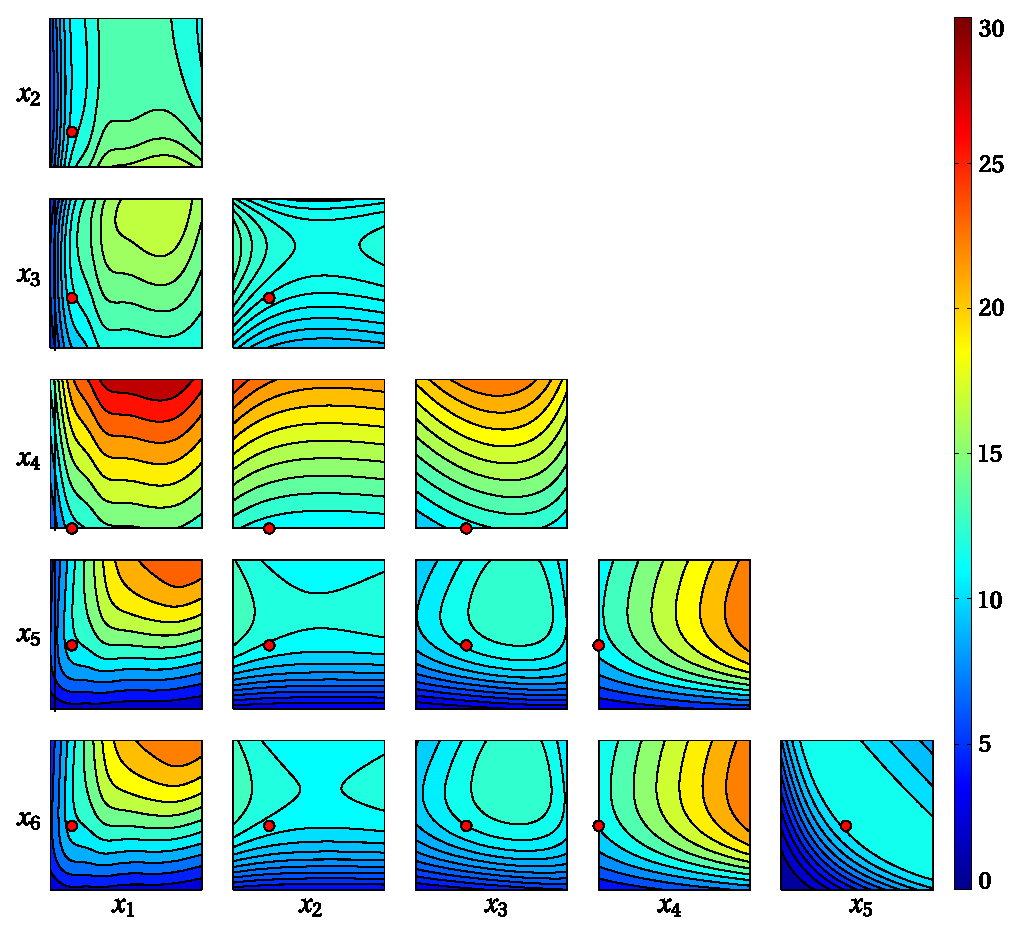
\includegraphics[scale=0.8]{../img/Optimizacion_del_Diseno/flandscape_labeled.eps}
\caption{Visualización de la función objetivo a través del metamodelo obtenido, por medio de la gráfica de contorno alrededor del punto de diseño inicial.}
\label{fig:flandscape}
\end{figure}
Como una guía adicional para la evaluación de métodos que puedan ser aplicables al problema, se puede realizar un análisis cualitativo de la función objetivo, utilizando la red neuronal que se obtuvo como metamodelo para la misma. Si se define $\mathbf{x}_0$ como el diseño inicial del MLR, entonces puede obtenerse una serie de gráficas de contorno de la función objetivo, fijando 4 variables con los valores de $\mathbf{x}_0$ y dejando las dos variables restantes libres entre los rangos definidos para cada una. En total, con 6 variables de diseño, se obtienen 15 combinaciones posibles, como se muestra en la Fig. \ref{fig:flandscape}, en donde se ha resaltado el punto de diseño inicial con un punto rojo.

La observación de estas gráficas de contorno permite observar varias características de la función objetivo alrededor del punto de diseño inicial. En primera instancia, no se observa un comportamiento multimodal, sino regiones de valores máximos definidas y puntos de silla. En algunas de las gráficas de contorno puede observarse un comportamiento casi convexo, aunque esta generalización puede no ser aplicable sobre todo el espacio de diseño. Es claro, sin embargo, que la función es suave en la región analizada, debido a que no se presentan discontinuidades en ninguna de las gráficas de contorno.

Con respecto al problema de optimización, se concluyó entonces que, debido al uso de un metamodelo, la función objetivo puede ser evaluada rápidamente; el panorama de la función objetivo alrededor del punto inicial no muestra la existencia de varios máximos y mínimos locales; la función objetivo es suave, y las restricciones en las variables de decisión son lineales, como se definieron en el capítulo 3.

Los resultados obtenidos de la revisión literaria y las anteriores propiedades del problema motivaron a la aplicación de tres métodos de optimización: 
\begin{itemize}
\item La \textbf{programación cuadrática secuencial} (PCS), un método determinístico que se seleccionó debido al comportamiento suave observado en la función objetivo.
\item El \textbf{algoritmo genético} (AG), un método de búsqueda estocástico basado en la dinámica de las poblaciones, seleccionado por su popularidad en el área de la optimización \cite{tenne2010}.
\item El algoritmo de \textbf{forrajeo de bacterias} (AFB), que combina conceptos de dinámicas poblacionales junto con enjambres de partículas, seleccionado debido a que su aplicación en la optimización de máquinas eléctricas no ha sido ampliamente explorada \cite{duan2013}.
\end{itemize}

\section{Evaluación de métodos de optimización}
A continuación se realiza una breve descripción de los métodos de optimización considerados en el presente trabajo.

\subsection{Programación cuadrática secuencial}
La PCS puede ser aplicada en problemas con restricciones lineales o no lineales, cuya función objetivo es no lineal \cite{nocedal1999}. Las características de la función objetivo mencionadas en la sección anterior indican que el problema tratado puede ser solucionado por medio de este último método, el cual ha sido utilizado en trabajos relacionados con la optimización de máquinas eléctricas \cite{raminosoa2006,astrid2014,barhoumi2016}. El problema de programación no lineal al que puede ser aplicada PCS secuencial puede expresarse como
\begin{align*}
\text{min } &f(\mathbf{x})\\
\text{sujeto a } &c_i(\mathbf{x}) = 0,\\
&c_d(\mathbf{x}) \geq 0
\end{align*}
donde $f:\mathbb{R}^n\rightarrow\mathbb{R}$ es una función suave, y $c_i(\mathbf{x})$ y $c_d(\mathbf{x})$ corresponden a las restricciones de igualdad y desigualdad, respectivamente, las cuales son propiedades que se encuentran en el problema de optimización tratado. 

La PCS formula y resuelve un sub-programa de programación cuadrática a partir de un punto inicial, que es utilizado para generar el valor en una siguiente iteración. En combinación con métodos más avanzados como regiones de confianza (conocidos como \textit{trust-region methods} en la literatura), puede obtenerse la convergencia para problemas no convexos \cite{nocedal1999}.

\subsection{El algoritmo genético}
El AG es un método de optimización basado en la teoría de la evolución. A partir de una codificación de las variables de decisión del problema, el AG aplica tres operadores a un conjunto de valores de las variables de decisión (la ``población'') de manera iterativa: \textbf{selección}, \textbf{cruce} y \textbf{mutación} \cite{goldberg1989}. Una de las principales ventajas del AG es que su operación no depende de la forma en que la función objetivo es evaluada, de expresiones analíticas o de la existencia de derivadas, ya que únicamente trabaja con los valores de la función objetivo.

El AG ha sido utilizado satisfactoriamente en optimización en la optimización de máquinas eléctricas a partir del FEM \cite{cassimere2009,dinardo2015,tuvsar2007}, o por medio de un metamodelo \cite{hasanien2010b}.

El AG opera inicialmente definiendo una población, donde cada individuo es evaluado a través de la función objetivo\footnote{Aunque puede trabajarse directamente con los valores de la función objetivo, es posible explorar transformaciones de la misma para evitar problemas de convergencia prematura (véase la sección \textit{Fitness Scaling} del capítulo 3 en \cite{goldberg1989}).}, donde el valor obtenido representa una figura de mérito, o una medición del desempeño de cada individuo, que define la ``aptitud''. Dependiendo de la definición del problema de optimización, los individuos más aptos pueden ser aquellos para los cuales la función objetivo produce valores más altos, en problemas de maximización, o valores más bajos en problemas de minimización.

Una vez cada individuo ha sido evaluado, se pasa a la aplicación de los operadores genéticos:
\begin{itemize}
\item \textbf{Selección:} los mejores individuos se seleccionan para la siguiente etapa, y el resto es eliminado.
\item \textbf{Cruce:} se seleccionan pares de individuos que son combinados. Esta operación puede realizarse de diferentes maneras, dependiendo de la codificación que se utilice, sea binaria o real \cite{herrera1998}.
\item \textbf{Mutación:} de acuerdo a cierta probabilidad, alguno de los parámetros de los individuos producto del cruce cambia de forma aleatoria, dentro de los valores establecidos para el problema.
\end{itemize}

La aplicación sucesiva de los tres operadores descritos constituye una ``generación'' de individuos. El proceso es repetido sucesivamente hasta que se cumple algún criterio, como un valor especificado de la función objetivo, un número de generaciones, entre otros.

\subsection{Optimización basada en forrajeo de bacterias}

A partir de la observación del comportamiento de la bacteria \textit{Escherichia Coli}, el AFB abstrae una serie de operaciones que pueden ser implementadas computacionalmente \cite{passino2002}. Este algoritmo es de interés debido a que aunque ha sido utilizado ampliamente en el control e identificación de sistemas \cite{precup2014,precup2014b}, su uso en la optimización de máquinas eléctricas, específicamente de motores lineales, no ha sido explorado de la misma forma \cite{duan2013,sakthivel2010}. Por otro lado, es una metaheurística similar al AG, pero que incluye otros fenómenos relacionados con la interacción entre los individuos de la población a medida que el espacio de diseño es explorado.

El primer paso del algoritmo, al igual que en el AG, consiste en la evaluación de la función objetivo, añadiendo el efecto de interacción entre las bacterias. A esto sigue la aplicación de diferentes operaciones:

\begin{itemize}
\item \textbf{Giro y movimiento:} (también conocido como \textit{quemotaxis}) cada bacteria da un pequeño paso aleatorio en cualquier dirección del espacio de diseño. Sólo aquellas bacterias para las cuales la superficie de nutrientes en la que se encontraban mejoró, son movidas, y el resto permanecen en el mismo lugar.
\item \textbf{Reproducción:} la mitad de las bacterias ubicadas en las regiones más bajas de la superficie de nutrientes muere, y las sobrevivientes se dividen en dos.
\item \textbf{Dispersión y eliminación:} existen algunos eventos durante la vida de una bacteria que pueden cambiar súbitamente su posición, como la dispersión o la eliminación por agentes externos. Dentro del algoritmo, esto se traduce como un cambio aleatorio en la posición de una bacteria.
\end{itemize}

Según resalta Passino en \cite{passino2002}, en la naturaleza, estos eventos ocurren en este orden, de mayor frecuencia a menor frecuencia, respectivamente, por lo que se sugiere una implementación de ciclos anidados donde el ciclo interior, ocurriendo con mayor frecuencia, es el de quemotaxis, el ciclo intermedio el de reproducción, y el ciclo exterior el de dispersión y eliminación.

\section{Metodología}
La aplicación de los tres métodos descritos anteriormente se realizó por medio de Matlab. Para el caso de la PCS se utilizó la función \texttt{fmincon}, especificando el algoritmo \texttt{sqp} (de \textit{Sequential Quadratic Programming}). Debido a que esta función encuentra un mínimo local, la salida del metamodelo se multiplicó por -1 para obtener un máximo de la función objetivo.

El AG y AFB, por otro lado, se implementaron completamente por medio de código, en las funciones \texttt{runga} y \texttt{runbf}, respectivamente, que pueden examinarse en el apéndice C. Con el fin de aprovechar las ventajas de la implementación de la red neuronal del metamodelo, que permite operar con matrices de entrada para evaluar varios diseños al mismo tiempo, se hizo énfasis en operar igualmente con matrices en estos dos algoritmos, de forma que su ejecución fuera mucho más eficiente.

El AG implementado hace necesaria la especificación de 5 parámetros, mientras que el AFB requiere de 11 parámetros. Estos parámetros están relacionados explícitamente con el funcionamiento de cada algoritmo (como el tamaño de la población, el número de generaciones y probabilidades de operaciones, entre otros), que fueron sintonizados manualmente de forma que se los algoritmos convergieran y evitando obtener extremos locales de forma prematura, debido a que no existe una regla aplicable a problemas específicos para determinar los parámetros de cada algoritmo \cite{goldberg1989,passino2002}.

Con el fin de caracterizar la aleatoriedad presente en el AG y el AFB, estos se ejecutaron 100 veces cada uno. 

Para la inicialización en los tres métodos se utilizó el diseño inicial. Cabe destacar que el valor de la función objetivo para el diseño inicial es de 11.6 N$^2$/W (newton al cuadrado por vatio).

\section{Resultados}
Mientras la programación cuadrática secuencial, al ser un método determinístico, llega a un mismo mínimo local si es ejecutado varias veces, los elementos probabilísticos de los AG y AFB producen resultados ligeramente diferentes. Sin embargo, cualitativamente, se obtuvo prácticamente el mismo resultado en los tres casos: el mejor diseño obtenido produjo un valor en la funcíón objetivo alrededor de 80 N$^2$/W, aproximadamente 8 veces más alto que el valor del diseño inicial. 

En la Fig. \ref{fig:resultshist} se muestran los histogramas para las 100 ejecuciones del AG y el AFB, junto con una línea que indica el resultado obtenido por medio de la PCS. Los histogramas muestran que, de acuerdo a los parámetros fijados en cada algoritmo, el AG presenta una mayor varianza en el valor de la función objetivo del diseño optimizado que el AFB. Además, los valores producidos por el AFB son en promedio mayores a los producidos por el AG. No obstante, este es un comportamiento que es altamente dependiente de los parámetros de cada algoritmo (probabilidades de cruce, mutación, movimiento, dispersión, etc.). Los valores máximos obtenidos por estos dos fueron bastante cercanos, de 78.3 en el AG y 78.4 en el AFB, mientras que el mayor valor fue obtenido por la PCS, con 78.6. Sin embargo, los tres métodos coinciden en un mismo diseño, ya que las diferencias entre los diseños que producen son prácticamente negligibles a la hora de construir el MLR con las dimensiones especificadas, como se muestra en la Tabla \ref{table:designsparams}.

\begin{figure}[t]
\centering
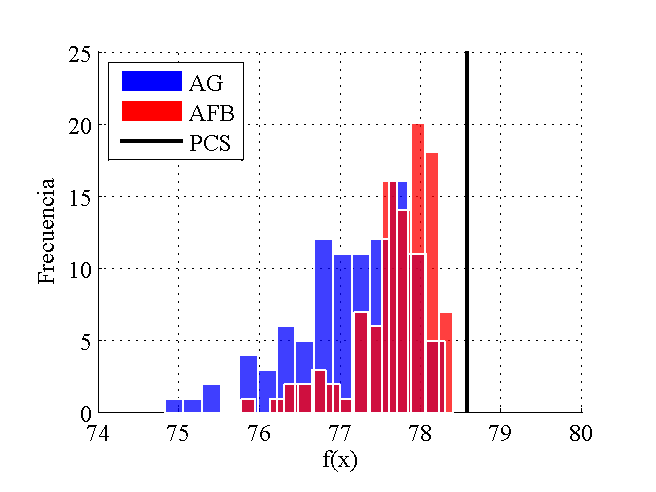
\includegraphics[scale=0.7]{../img/Optimizacion_del_Diseno/resultshist.eps}
\caption{Valores de la función objetivo obtenidos para cada uno de los métodos.}
\label{fig:resultshist}
\end{figure}

\begin{table}[t]
\centering
\caption{Parámetros de los diseños del MLR obtenidos.}
\label{table:designsparams}
\begin{tabular}{c c c c c}\hline
Variable & Inicial & PCS & AG & AFB\\
\hline\hline
Paso polar (cm) & 6 & 12.00 & 11.80 & 11.99\\
Ancho del motor (cm) & 7.14 & 5.00 & 5.20 & 5.01\\
Razón $\beta_s/\tau_s$ & 0.5 & 0.66 & 0.65 & 0.66\\
Alto de ranura (cm) & 2 & 4.00 & 3.97 & 3.99\\
Corriente de fase (A) & 2.7 & 5.00 & 4.84 & 4.99\\
Vueltas por bobina & 57 & 100 & 100 & 97
\end{tabular}
\end{table}

El efecto de los AG y AFB sobre cada una de sus poblaciones puede observarse al guardar el valor de la función objetivo en el mejor y en el peor caso, para cada generación en el caso del AG, y en cada ciclo de quemotaxis para el AFB. Estos resultados se muestran en la Fig. \ref{fig:gabfevolution}, donde además se han señalado con líneas gruesas horizontales los valores de la función objetivo para el diseño inicial (en negro) y el diseño optimizado (en rojo). Estas líneas permiten visualizar cómo el valor de la función objetivo se incrementó considerablemente después de la aplicación de estos algoritmos.

En ambos casos, se han dibujado los valores de los peores individuos con una línea azul, y los de los mejores individuos con una línea roja. Los eventos en los que los peores individuos resultan en valores por debajo del promedio ilustran cambios drásticos producidos por mutaciones en el AG, y por eventos de dispersión en el AFB. La presencia de mayores cambios en el AG con respecto a aquellos en el AFB se debe a la forma en que estos son incluidos en el algoritmo: mientras las mutaciones pueden ocurrir con cierta probabilidad en cada generación del AG, los eventos de dispersión en el AFB sólo ocurren después de varios eventos de reproducción, cada uno con un número de eventos de quemotaxis.

\begin{figure}[t]
    \centering
    \begin{subfigure}[b]{0.49\textwidth}
    \centering
        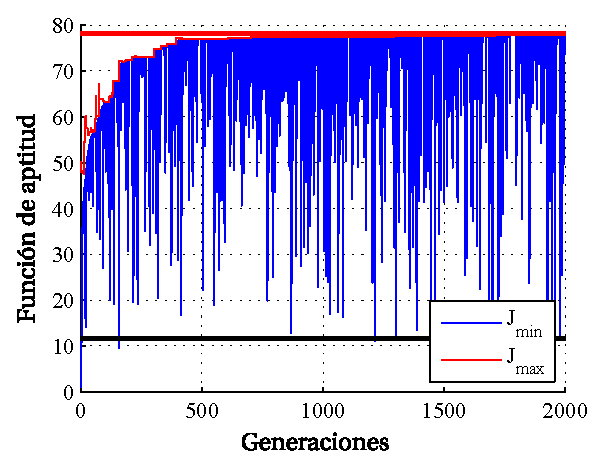
\includegraphics[scale=0.65]{../img/Optimizacion_del_Diseno/gaevolution.eps}
        \caption{AG}
        \label{fig:gaevolution}
    \end{subfigure}
    ~ %add desired spacing between images, e. g. ~, \quad, \qquad, \hfill etc. 
      %(or a blank line to force the subfigure onto a new line)
    \begin{subfigure}[b]{0.49\textwidth}
    \centering
        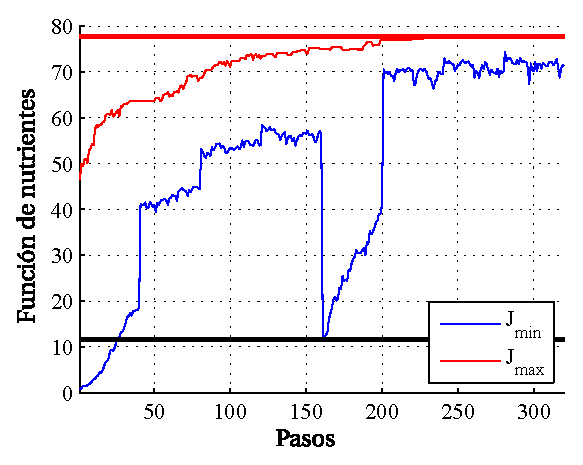
\includegraphics[scale=0.65]{../img/Optimizacion_del_Diseno/bfevolution.eps}
        \caption{AFB}
        \label{fig:bfevolution}
    \end{subfigure}
    \caption{Progreso del AG y el AFB.}\label{fig:gabfevolution}
\end{figure}

A pesar de que se hizo énfasis en una implementación del AG y el AFB que operara directamente con matrices, se observó que el tiempo de ejecución de estos dos fue de hasta cuatro veces el tiempo de ejecución de la PCS. Para cuantificar esta observación, se realizó un conteo del número de evaluaciones de la función objetivo requerido por cada método para llegar al diseño optimizado. Los resultados fueron los siguientes:

\begin{table}[h]
\centering
\begin{tabular}{c c}
\textbf{Método} & \textbf{Evaluaciones}\\
PCS & 105\\
AG & 400 000\\
AFB & 86 670
\end{tabular}
\end{table}

Finalmente, de acuerdo a los resultados obtenidos en el proceso de optimización, se procedió a validar el diseño obtenido por medio del FEM. Los resultados obtenidos indicaron que el empuje producido por el diseño optimizado del motor es de 150 N, con una eficiencia del 51\%. Esto es una consecuencia directa de la prioridad dada al empuje en la definición de la función objetivo, y a que la corriente de fase se incluyó dentro de las variables de diseño. Teniendo en cuenta que los requisitos del motor especifican un empuje menor a 150 N, la corriente se redujo de 5 A (valor obtenido por medio de los métodos de optimización) a 2 A, donde el empuje producido por el motor es de 50 N, como es requerido, logrando finalmente una eficiencia de \textbf{68\%}.

\section{Conclusiones}
Al igual que durante la construcción de un metamodelo para la función objetivo, la revisión del estado del arte y la evaluación de diferentes métodos de optimización permitió verificar la ausencia de un método específico a seguir a la hora de resolver un problema de optimización, tal como enuncia el NFLT. Aunque los resultados obtenidos fueron similares, la PCS resultó ser en este caso un método mucho más eficiente (en términos del número de evaluaciones de la función objetivo) que el AG y el AFB, a pesar de que se buscaron parámetros de estos dos últimos algoritmos que aceleraran su convergencia. Teniendo en cuenta que la construcción del metamodelo hizo necesaria la evaluación de 2000 experimentos, se puede concluir que una estrategia más eficiente para problemas similares es la aplicación de la PCS directamente sobre el FEM como método de evaluación de la función objetivo. No obstante, los tres algoritmos cumplieron con el objetivo, y en un futuro es posible evaluar otros métodos que puedan ser más eficientes.

Aunque el uso de la PCS no garantiza un óptimo global en el espacio de diseño restringido, y no se ha probado que el óptimo obtenido sea en realidad global, el diseño obtenido presentó un desempeño superior al diseño inicial, pasando de una eficiencia de 32\% al 68\%, o un poco más del doble de la eficiencia. Este es un valor aceptable dentro de los rangos de eficiencia obtenidos para los MLR en trabajos relacionados (como se mostró en el capítulo 2).

A partir de los cambios entre el diseño inicial y el optimizado, se evidenció que el motor mejorado se obtuvo al incrementar el alto y el largo del motor, el tamaño de las ranuras y el número de vueltas por fase, mientras que el ancho se redujo, lo que permitió obtener el mismo empuje del diseño inicial, a un nivel menor de corriente y producir así, una eficiencia mayor.

\bibliographystyle{ieeetr}
\bibliography{../refs}